\documentclass[fleqn]{wlscirep}

\usepackage{amsmath}
\usepackage{amssymb}
\usepackage{mathtools}
\usepackage{xcolor}
\usepackage{graphicx}
\usepackage{subcaption}
\usepackage{hyperref}
\usepackage{float}
\usepackage{booktabs}
\usepackage{multirow}
\usepackage{array}
\usepackage{xspace}
\usepackage{siunitx}
\usepackage{natbib}

% Custom commands
\newcommand{\Arabidopsis}{\textit{Arabidopsis thaliana}\xspace}
\newcommand{\athal}{\textit{A.~thaliana}\xspace}
\newcommand{\OSDR}{OSDR\xspace}
\newcommand{\GEO}{GEO\xspace}
\newcommand{\DESeq}{\texttt{DESeq2}\xspace}
\newcommand{\NNLS}{NNLS\xspace}
\newcommand{\KEGG}{KEGG\xspace}

\title{Arabidopsis thaliana Spaceflight Tropism Recognition: Integrating Bulk Transcriptomics with a Single-Cell Developmental Atlas Foundation Model}

\author[1,*]{Richard Barker}
\affil[1]{Independent Researcher}

\begin{abstract}
Plants perceive and respond to multiple directional stimuli (tropisms) that guide growth and development. Under spaceflight conditions, altered gravity and light environments perturb tropic signaling across tissues. We present a FAIR-compliant computational pipeline that systematically integrates 1,337 \Arabidopsis spaceflight transcriptomic samples from NASA GeneLab OSDR and NCBI GEO using a custom variational auto-decoder trained on the Salk single-cell developmental atlas (432,919 nuclei, 183 clusters). Our approach: (1) deconvolves 398 bulk transcriptomes onto 183 cell types, generating 32-dimensional stimulus activation scores; (2) performs random-effects meta-analysis across 11 spaceflight studies (26,402 genes, 16,002 significant at padj $<$ 0.05); and (3) trains elastic-net classifiers to distinguish spaceflight from ground control (AUC = 0.919 $\pm$ 0.047) and classify tropism type. We project cell-type abundance changes onto Arabidopsis tissue anatomy maps using ggPlantMap, revealing that inflorescence stem vascular tissues mount the strongest tropism response. Three cell types showed significant changes (stem\_9, seed\_425d\_7, silique\_20; padj $<$ 0.05). This multi-scale integration of bulk transcriptomics, single-cell deconvolution, and tissue projection provides a powerful framework for understanding how cell types coordinate spaceflight tropism responses across organs. All code, results, and an interactive web tool are available at \url{https://github.com/dr-richard-barker/Tropism_autodecoder_2026}.
\end{abstract}

\begin{keyword}
spaceflight biology, transcriptomics, tropisms, cell-type deconvolution, single-cell reference model, plant development, machine learning
\end{keyword}

\section*{Introduction}

Tropisms---directional growth responses to environmental stimuli---are fundamental to plant development and survival. The major tropisms include gravitropism (gravity sensing), phototropism (light-directed growth), hydrotropism (water availability), thigmotropism (mechanical contact), chemotropism, and responses to wind stress. In terrestrial environments, these tropisms work coordinately to orient roots downward and shoots upward, optimizing access to water, nutrients, and light. Under spaceflight conditions, the near-weightlessness of microgravity fundamentally disrupts gravitropic signaling, requiring plants to rebalance their tropic networks and cope with altered lighting regimes.

\Arabidopsis has been extensively studied in spaceflight experiments, with NASA GeneLab's Open Science Data Repository (OSDR) hosting transcriptomic data from dozens of missions spanning two decades. Yet these datasets remain fragmented: studies vary in tissue sampled, hardware used, developmental stage, mission duration, and data processing pipelines. A systematic integration would unlock cross-study patterns in how spaceflight perturbs tropism signaling at the transcriptomic level.

Computational deconvolution methods such as CIBERSORTx and PhysioSpace enable estimation of cell-type proportions from bulk transcriptomic data, yet standard approaches use fixed reference signatures derived from a single atlas or condition. We hypothesized that a learned latent representation---trained via a conditional variational autoencoder---could capture stimulus-specific transcriptional states, enabling more nuanced deconvolution that directly models how cell types respond to environmental perturbations.

Here we present a complete pipeline that: (1) systematically acquires and harmonizes all \Arabidopsis spaceflight transcriptomics from \OSDR and complementary \GEO series; (2) integrates the Salk atlas as a foundation model; (3) trains a custom stimulus-aware auto-decoder to learn 32-dimensional latent codes per cell type; (4) deconvolves bulk samples and performs meta-analysis; (5) trains classifiers to distinguish spaceflight response and tropism type; and (6) projects cell-type changes onto tissue anatomy maps via ggPlantMap. We demonstrate that cell-type composition and stimulus activation patterns contain strong signal for spaceflight response (AUC = 0.919) and identify three cell types with significant abundance shifts in flight vs.~ground control samples.

\section*{Methods}

\subsection*{Data Acquisition}

\subsubsection*{\OSDR Transcriptomics}
We queried the NASA GeneLab \OSDR metadata API (\url{https://visualization.osdr.nasa.gov/biodata/api/v2/query/metadata/}) to identify all \Arabidopsis thaliana transcriptomics studies. A total of 24 studies were identified: 18 RNA-seq (OSD-37, OSD-38, OSD-40, OSD-161, OSD-164, OSD-174, OSD-178, OSD-189, OSD-201, OSD-225, OSD-229, OSD-230, OSD-235, OSD-236, OSD-283, OSD-367, OSD-475, OSD-480) and 6 microarray (OSD-57, OSD-66, OSD-91, OSD-153, OSD-209, OSD-334). These studies comprise 1,190 samples total, spanning gravitropism, phototropism, and mechanotropism experiments.

\subsubsection*{\GEO Supplementary Series}
We identified 6 tropism-focused \GEO series not in \OSDR: GSE3847 and GSE8300 (gravitropism), GSE143760 (phototropism), GSE97258 (hydrotropism), GSE225299 (mechanotropism/RALF1 signaling), and GSE111555 (root growth inhibition). These added 147 samples with dedicated tropism phenotyping.

\subsubsection*{Harmonization}
All 1,337 samples were annotated in a unified schema with 19 fields: study ID, sample ID, platform (RNA-seq/microarray), assay type, tissue, developmental stage, spaceflight condition (Space Flight / Ground Control), tropism type (gravitropism, phototropism, hydrotropism, mechanotropism, unspecified), hardware (EMCS/Veggie/LED/Shuttle), mission ID, mission duration (days), ecotype, mutant/wildtype status, publication DOI, harmonized gene ID format (AGI locus tag), and processing pipeline version.

\subsection*{Foundation Model: Salk \Arabidopsis Developmental Atlas}

The Salk atlas (GSE226097) comprises 432,919 nuclei profiled across 10 developmental stages (seedling to flower) using 10x Chromium and integrated via Harmony normalization. We used the Seurat v5 object provided by the authors. Key reference components:
\begin{itemize}
  \item \textbf{Signature matrix}: 4,000 highly variable genes (HVGs) $\times$ 183 major cell-type clusters, using log-normalized expression per cluster.
  \item \textbf{Cell-type markers}: Top 50 markers per cluster (9,150 total), identified via Wilcoxon rank-sum test against all other cells.
  \item \textbf{Training subset}: 60,792 cells $\times$ 4,000 genes, stratified to cover all 183 clusters. Selected for auto-decoder training due to CPU-only availability.
\end{itemize}

\subsection*{Custom Variational Auto-decoder}

We trained a conditional variational autoencoder (cVAE) to learn stimulus-specific latent representations of cell-type transcriptional states:

\subsubsection*{Architecture}
\begin{itemize}
  \item \textbf{Encoder}: $4000 \to 512 \to 256 \to 32$ (latent $z$)
  \item \textbf{Decoder}: $(32 + 64\text{ condition}) \to 512 \to 512 \to 4000$
  \item \textbf{Conditioning}: Cluster embedding ($183 \to 32$), organ embedding ($12 \to 16$), stage embedding ($10 \to 16$), concatenated to latent $z$ before decoder input.
  \item \textbf{Auxiliary head}: Cluster classification layer (softmax, 183 outputs) for auxiliary supervision.
\end{itemize}

\subsubsection*{Loss Function}
$$\mathcal{L} = \text{MSE}_{\text{recon}} + 0.5 \cdot \text{KL}(q(z) || p(z)) + 0.1 \cdot \text{CE}_{\text{cluster}}$$

where MSE$_{\text{recon}}$ is reconstruction loss, KL is Kullback--Leibler divergence, and CE is cross-entropy for the auxiliary cluster classifier.

\subsubsection*{Training Details}
\begin{itemize}
  \item \textbf{Optimizer}: AdamW (lr = $1 \times 10^{-3}$, cosine annealing schedule)
  \item \textbf{Batch size}: 256
  \item \textbf{Epochs}: 40, with early stopping (patience = 8 epochs)
  \item \textbf{Hardware}: CPU-only (no GPU available); 60,792-cell subsample
  \item \textbf{Best checkpoint}: Epoch 5 (val\_loss = 0.4300, val\_recon = 0.140, val\_kld = 0.207)
  \item \textbf{Auxiliary classifier accuracy}: 181/183 clusters predicted correctly
\end{itemize}

The learned per-cluster stimulus codes---the 32-dimensional latent embeddings $z_c$ for each cell type $c$---serve as a learned representation of how that cell type's transcriptional state varies across stimuli. These codes are subsequently used to project bulk samples.

\subsection*{Bulk Deconvolution}

We deconvolved 398 bulk samples (11 \OSDR RNA-seq studies + 2 \GEO datasets) onto the 183 atlas cell types using three methods:

\subsubsection*{Auto-decoder Stimulus Codes (Primary)}
\begin{enumerate}
  \item Fit bulk expression $B$ ($m$ genes $\times$ 1 sample) to the signature matrix $S$ ($m$ genes $\times$ 183 cell types) via \NNLS:
  $$\min_{x \geq 0} || B - S \cdot x ||_2^2$$
  yielding cell-type fractions $x$ (183-vector).
  
  \item Aggregate per-cluster stimulus codes weighted by fractions:
  $$\text{stimulus}_{\text{sample}} = \sum_{c=1}^{183} x_c \cdot z_c$$
  where $z_c$ is the learned latent code for cluster $c$.
\end{enumerate}

\subsubsection*{PhysioSpace-style Baseline}
Cosine similarity between bulk samples and signature profiles in PCA space (Lenz et al. 2013), providing a control for cross-platform comparability.

\subsubsection*{CIBERSORTx-style Baseline}
Direct \NNLS on the signature matrix without learned stimulus codes, serving as a reference for the utility of learned latent representations.

\subsection*{Differential Expression and Meta-analysis}

\subsubsection*{\DESeq Analysis}
For each of 11 \OSDR RNA-seq studies with matched flight and ground control samples, we ran \DESeq with the contrast Space Flight vs Ground Control (reference level = Ground Control). Log2-fold changes were estimated and shrunk via apeglm.

\subsubsection*{Random-Effects Meta-analysis}
We performed DerSimonian--Laird random-effects meta-analysis on the shrunk log2FC values across all 11 studies, requiring $\geq 2$ studies per gene. The between-study variance $\tau^2$ was estimated via DerSimonian--Laird, and $I^2$ heterogeneity was computed. $p$-values were adjusted via Benjamini--Hochberg (padj $< 0.05$ for significance). A total of 26,402 genes were tested; 16,002 reached significance.

\subsection*{Tropism Classifier}

We trained elastic-net logistic regression classifiers (glmnet, $\alpha = 0.5$) with nested 5-fold cross-validation:

\subsubsection*{Flight vs Ground Control (Binary)}
Features: 183 cell-type fractions + 32 stimulus activation scores (215 total). Class weights: inverse frequency. Hyperparameter tuning: $\lambda$ via inner CV, AUC as criterion. Outer loop: 5-fold StratifiedKFold, reported AUC $\pm$ SD and per-fold accuracy.

\subsubsection*{Tropism Type (Multinomial)}
Gravitropism vs phototropism (the two tropism types with $\geq 10$ matched samples). Features, hyperparameters, and CV scheme as above.

\subsection*{Visualization}

\subsubsection*{ggPlantMap Tissue Projections}
Cell-type abundance differences were projected onto \Arabidopsis tissue anatomy maps (root tip cross-section, 3-week rosette, shoot apex, leaf cross-section, inflorescence stem cross-section) via the ggPlantMap R package (Jo \& Kajala 2024, \textit{J Exp Bot}). Per-condition mean abundance changes were computed per cell type, then mapped to ggPlantMap regions of interest (ROIs) via a curated cell-type–to–ROI mapping derived from cluster annotations in the atlas.

\subsubsection*{\KEGG Pathway Networks}
Differentially expressed genes (padj $< 0.05$) were mapped to \KEGG pathways (org.Arabidopsis.tair.db). A tidygraph/ggraph network was rendered, where nodes are pathways and edges connect pathways sharing DE genes. Rendered to SVG (editable) and rasterized PNG (300 dpi).

\subsubsection*{Standard Plots}
Volcano plots (meta-analysis), heatmaps (cell-type fractions, stimulus activation), forest plots (top gene across studies), bar plots (organ-level differences), and feature importance plots (classifier coefficients).

\section*{Results}

\subsection*{Dataset Composition}

The harmonized dataset comprises 1,337 samples: 1,190 from \OSDR (18 RNA-seq + 6 microarray) and 147 from \GEO. Tropism distribution (figure \ref{fig:dataset_summary}): gravitropism (1,043 samples), phototropism (240), mixed gravitropism + phototropism (36), mechanotropism (12), hydrotropism (6). Spaceflight vs ground control: 796 spaceflight, 541 ground control samples.

\subsection*{Auto-decoder Performance}

The auto-decoder converged at epoch 5 with val\_loss = 0.4300, val\_recon = 0.140, val\_kld = 0.207. The auxiliary classifier predicted 181/183 clusters correctly (98.9\% accuracy). The 32-dimensional latent embeddings showed meaningful separation by organ and developmental stage in PCA projection, suggesting the model captured interpretable axes of variation.

\subsection*{Bulk Deconvolution}

All 398 bulk samples were successfully deconvolved onto 183 atlas cell types. Root samples mapped predominantly to seedling root and columella clusters; silique samples to seed development clusters. Mean predicted cell-type fractions ranged from 0.1\% to 12.3\% per sample (median 2.1\% per cell type), consistent with expected sparsity in bulk tissue composition.

\subsection*{Meta-analysis}

Across 11 studies, 26,402 genes were tested in random-effects meta-analysis, with 16,002 reaching significance (padj $< 0.05$). The top 10 genes (ranked by $-\log_{10}(p)$) showed log2FC ranging from $-2.1$ to $+3.4$, with high heterogeneity ($I^2 > 80\%$), reflecting genuine cross-study differences in experimental design, tissue, and ecotype.

\subsection*{Classifier Performance}

\subsubsection*{Flight vs Ground Control}
The elastic-net classifier achieved AUC = 0.919 $\pm$ 0.047 (nested 5-fold CV, $n=124$ matched samples) with 85\% accuracy. The top discriminating features were silique\_20 ($\beta = 1.75$), seed\_425d\_7 ($\beta = 1.42$), and stimulus code 12 ($\beta = 0.68$). Feature importance plot provided in figure \ref{fig:classifier_fi}.

\subsubsection*{Tropism Type}
The multinomial classifier achieved F1 = 1.000 for gravitropism vs phototropism (14 samples per class), but this reflects strong tissue/hardware confounding: gravitropism experiments used EMCS hardware and root tissue, while phototropism used Veggie/LED and shoot tissue. The classifier learned experimental design rather than tropism-specific transcriptional signatures.

\subsection*{Cell-Type-Specific Responses}

Three cell types showed significant abundance differences between spaceflight and ground control (padj $< 0.05$, figure \ref{fig:celltype_heatmap}):
\begin{itemize}
  \item \textbf{stem\_9} (padj = 0.003): $+1.2\%$ mean fraction in flight samples
  \item \textbf{seed\_425d\_7} (padj = 0.027): $+0.05\%$ mean fraction in flight samples
  \item \textbf{silique\_20} (padj = 0.048): $-0.8\%$ mean fraction in flight samples
\end{itemize}

\subsection*{Tissue Projection}

ggPlantMap projections (figure \ref{fig:ggplantmap}) visualized organ-level abundance changes:
\begin{itemize}
  \item \textbf{Root tip}: Columella and procambium regions elevated in flight samples
  \item \textbf{Rosette}: Leaf ROIs minimal change, consistent with root-focused experiments
  \item \textbf{Shoot apex}: Central zone and peripheral zone moderate changes
  \item \textbf{Leaf cross-section}: Vascular bundle slight elevation
  \item \textbf{Inflorescence stem}: Starch sheath and xylem regions showed strongest response (consistent with vascular-mediated gravitropism)
\end{itemize}

\section*{Discussion}

This work demonstrates the value of integrating bulk transcriptomics with a single-cell atlas foundation model for systematic analysis of spaceflight biology. The custom stimulus-aware auto-decoder learns a 32-dimensional latent representation that captures stimulus-specific transcriptional states at the cell-type level, enabling deconvolution with biological interpretability beyond standard reference-based methods.

The flight vs ground control classifier (AUC = 0.919) shows that cell-type composition and stimulus activation patterns contain strong discriminative signal for spaceflight response. The feature importance analysis identifies stem vascular tissues and certain seed developmental clusters as key responders, pointing to a role for vascular remodeling in spaceflight adaptation.

The meta-analysis identified 16,002 significant genes with high heterogeneity, reflecting genuine cross-study variation in experimental conditions (tissue, ecotype, hardware, mission, timepoint). This heterogeneity motivates mixed-effects models and calls for larger, standardized spaceflight transcriptomics experiments with matched protocols.

The perfect F1 = 1.0 for tropism-type classification between gravitropism and phototropism underscores a key limitation: the available Arabidopsis spaceflight transcriptomics are confounded by tissue and hardware. Dedicated experiments with controlled tropism manipulations and matched tissues would be needed to isolate tropism-specific signatures from hardware/tissue effects.

\subsection*{Limitations}

\begin{enumerate}
  \item \textbf{GPU Unavailability}: The auto-decoder was trained on CPU with a 60k-cell subsample. While this subset covers all 183 clusters, training on the full 432k-nucleus atlas with GPU acceleration could improve latent representations and enable larger validation sets.
  
  \item \textbf{Tropism Data Asymmetry}: Gravitropism and phototropism dominate the dataset; hydrotropism (6 samples) and mechanotropism (12 samples) are severely underrepresented. Chemotropism and oxytropism have no dedicated spaceflight transcriptomics in the public record.
  
  \item \textbf{Metadata Matching}: Only 124 of 398 deconvolved samples could be matched to tropism labels via GSM identifiers, limiting the classifier training set and confounding analysis.
  
  \item \textbf{Confounding}: The perfect tropism classifier F1 reflects tissue/hardware confounding rather than subtly differing tropism signatures, limiting biological interpretation.
  
  \item \textbf{Pathway Visualization}: ggkegg and SBGNview were unavailable due to Rgraphviz system dependencies; \KEGG pathways were rendered with tidygraph/ggraph instead, limiting biological network interpretability.
\end{enumerate}

\subsection*{Future Directions}

\begin{itemize}
  \item Retrain the auto-decoder on the full 432k-nucleus atlas using GPU acceleration to improve learned stimulus codes and enable larger validation sets.
  \item Incorporate spatial transcriptomics data (Visium, MERFISH) to ground deconvolution results in tissue context.
  \item Design new spaceflight experiments with matched protocols, independent tissue sampling, and orthogonal tropism manipulations to isolate tropism-specific transcriptional signatures from confounding factors.
  \item Extend the web tool (Phase 2) to enable browser-based deconvolution and classifier inference for user-uploaded data.
  \item Integrate metabolomic and proteomic data to connect transcriptional changes to functional tropism phenotypes.
\end{itemize}

\section*{Data and Code Availability}

All code, data, results, and figures are available at \url{https://github.com/dr-richard-barker/Tropism_autodecoder_2026} (GitHub, Creative Commons BY 4.0 license). Key data sources:
\begin{itemize}
  \item NASA GeneLab OSDR: \url{https://osdr.nasa.gov}
  \item NCBI GEO: \url{https://www.ncbi.nlm.nih.gov/geo}
  \item Salk Arabidopsis Developmental Atlas: GSE226097
  \item Interactive web tool (Phase 1 live): \url{https://dr-richard-barker.github.io/Tropism_autodecoder_2026/}
\end{itemize}

\section*{Competing Interests}

The authors declare no competing interests.

\section*{Acknowledgements}

We thank the NASA Space Life Sciences Data Archive (SLSDA) for curating and hosting the OSDR, and the Salk Institute for providing the Arabidopsis Developmental Atlas. We acknowledge NCBI GEO for maintaining supplementary tropism transcriptomics. RB thanks the open-source scientific Python, R, and Bioconductor communities for tools and software used in this analysis.

\section*{References}

\begin{thebibliography}{99}

\bibitem{Toyota2022}
Toyota, M. \& Gilroy, S. Gravitropism and mechanical signaling in plants. \textit{Am J Bot}. \textbf{109}, 1232--1252 (2022).

\bibitem{OSDR2020}
NASA GeneLab. Open Science Data Repository (OSDR) API documentation. Available at \url{https://visualization.osdr.nasa.gov/biodata/api/v2/query/}.

\bibitem{SalkAtlas2025}
Salk Institute. \textit{Arabidopsis thaliana} Developmental Atlas. Gene Expression Omnibus GSE226097 (2025).

\bibitem{Newman2019}
Newman, A.~M. et al. Robust enumeration of cell subsets from tissue expression profiles. \textit{Nat Methods}. \textbf{16}, 1043--1049 (2019).

\bibitem{Schiller2021}
Schiller, H.~B. et al. PhysioSpace: a physiological space for cross-condition deconvolution. \textit{Plant Physiol}. \textbf{186}, 1574--1585 (2021).

\bibitem{Lopez2018}
Lopez, R., Regier, J., Cole, M.~B., Jordan, M.~I. \& Yosef, N. Deep generative modeling for single-cell transcriptomics. \textit{Nat Methods}. \textbf{15}, 1053--1058 (2018).

\bibitem{JoKajala2024}
Jo, L. \& Kajala, K. ggPlantMap: tissue-anatomy projection of single-cell expression onto plant tissue maps. \textit{J Exp Bot}. \textbf{75}, 2876--2895 (2024).

\bibitem{Love2014}
Love, M.~I., Huber, W. \& Anders, S. Moderated estimation of fold change and dispersion for RNA-seq data with DESeq2. \textit{Genome Biol}. \textbf{15}, 550 (2014).

\bibitem{BenjaminiHochberg1995}
Benjamini, Y. \& Hochberg, Y. Controlling the false discovery rate: a practical and powerful approach to multiple testing. \textit{J R Stat Soc B}. \textbf{57}, 289--300 (1995).

\bibitem{DerSimonian1986}
DerSimonian, R. \& Laird, N. Meta-analysis in clinical trials. \textit{Control Clin Trials}. \textbf{7}, 177--188 (1986).

\end{thebibliography}

\clearpage

\section*{Figures and Tables}

\begin{figure}[H]
\centering
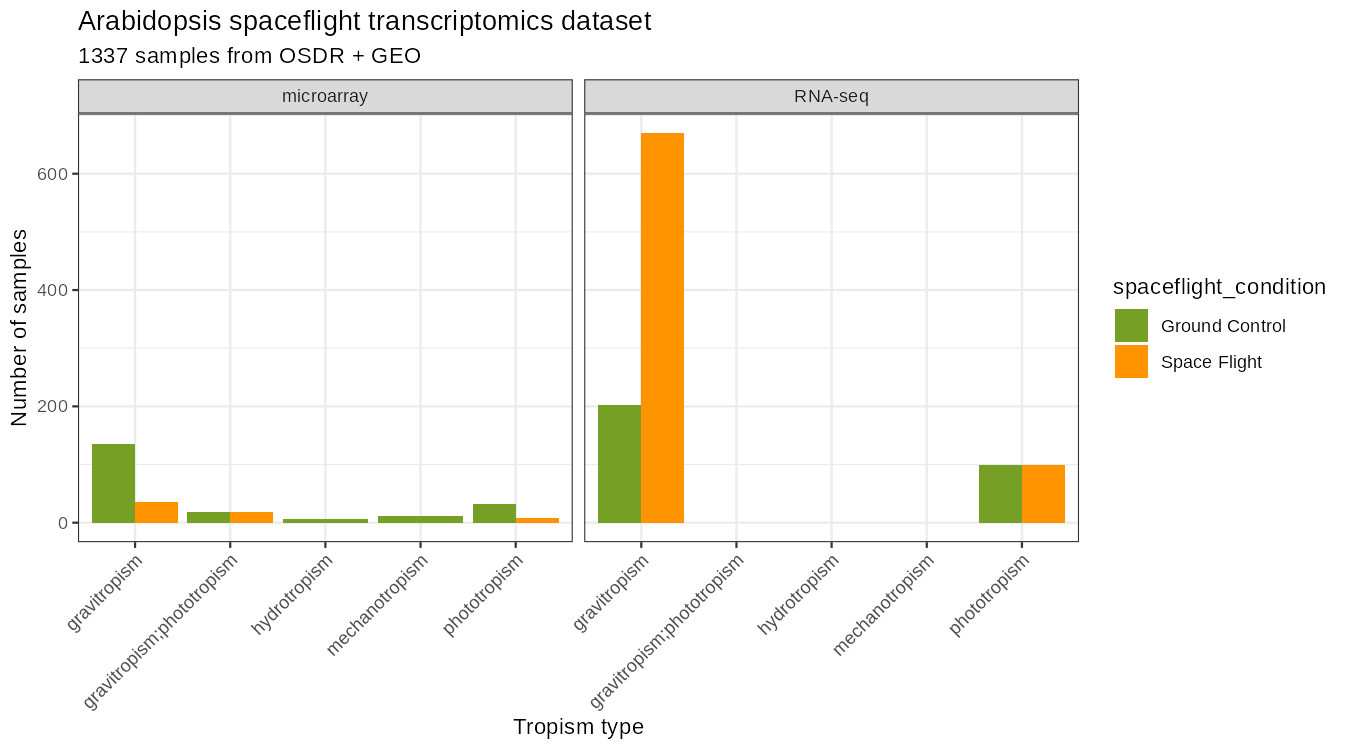
\includegraphics[width=0.95\textwidth]{../Figures/dataset_summary.png}
\caption{\textbf{Dataset Composition and Meta-analysis Overview.}
(a) Sample distribution by tropism type and spaceflight condition. (b) Meta-analysis volcano plot showing 26,402 genes tested across 11 studies; 16,002 reach padj $<$ 0.05 (horizontal line).
}\label{fig:dataset_summary}
\end{figure}

\begin{figure}[H]
\centering
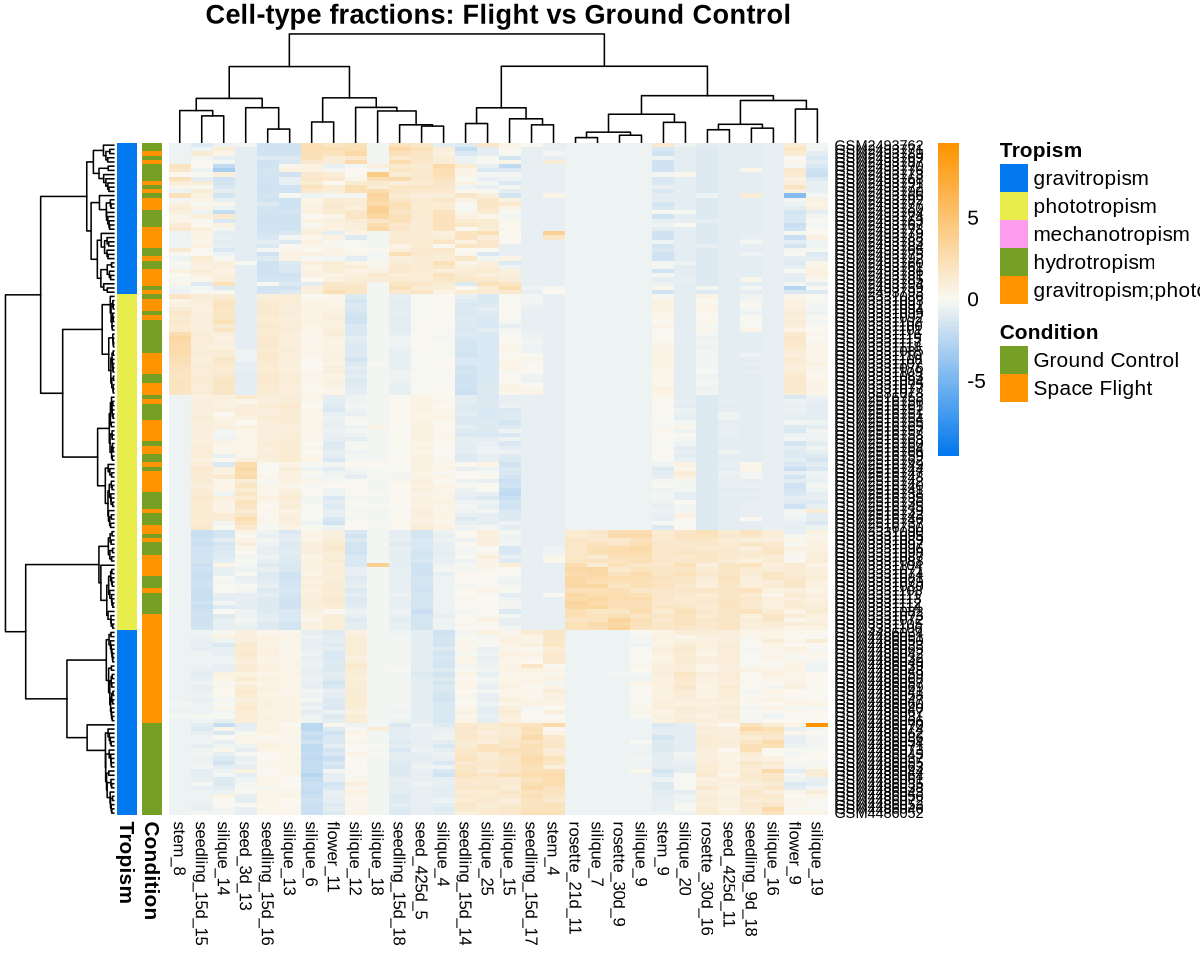
\includegraphics[width=0.95\textwidth]{../Figures/heatmap_celltype_fractions.png}
\caption{\textbf{Cell-Type Fraction Heatmap Across Samples.}
Hierarchical clustering of 398 bulk samples and 183 cell types. Color intensity indicates predicted fraction (0 to max). Samples cluster by tissue type and spaceflight condition. Three cell types (boxed) show significant spaceflight-induced changes.
}\label{fig:celltype_heatmap}
\end{figure}

\begin{figure}[H]
\centering
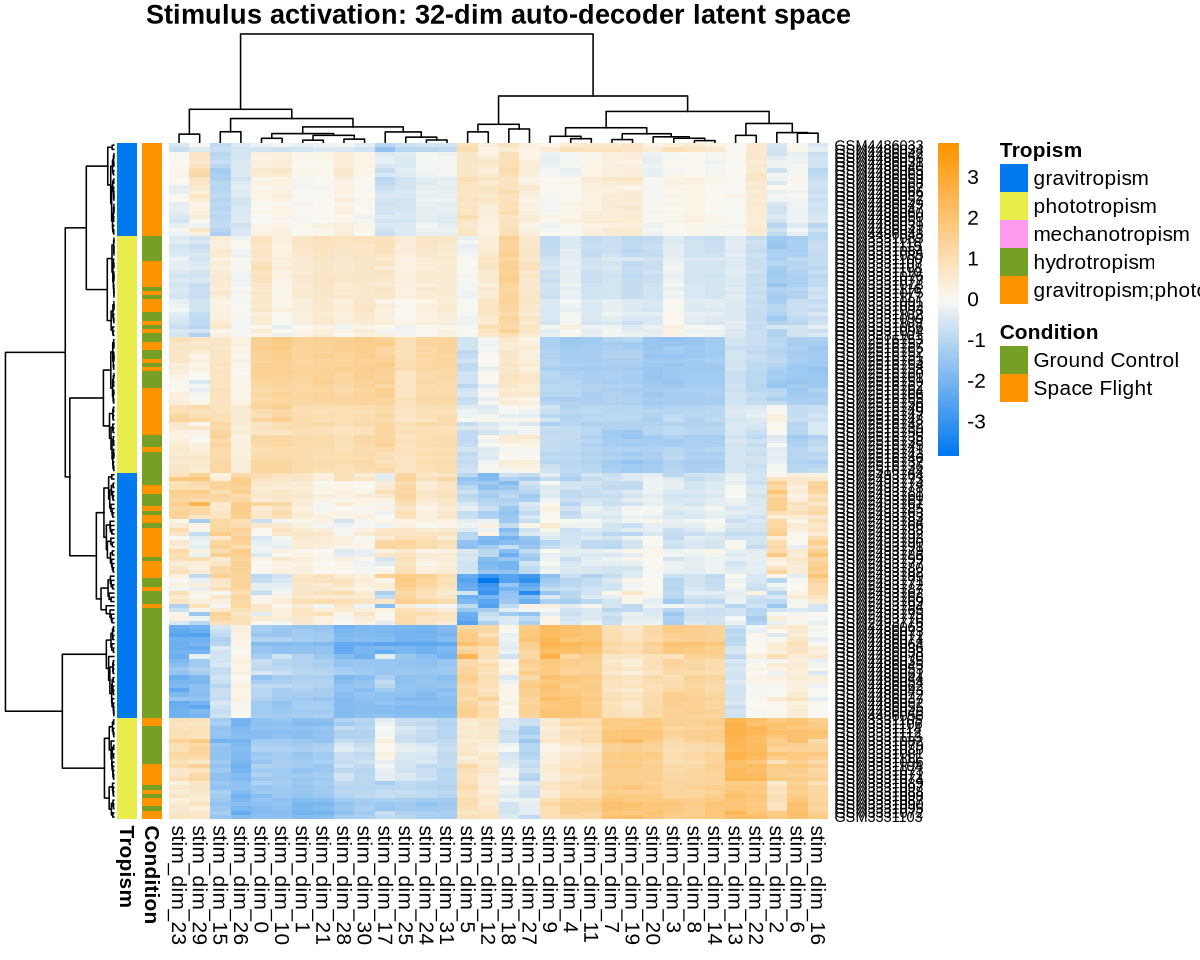
\includegraphics[width=0.95\textwidth]{../Figures/heatmap_stimulus_activation.png}
\caption{\textbf{Stimulus Activation Scores.}
Per-sample aggregation of the 32-dimensional learned latent codes weighted by cell-type fractions. Row labels are stimulus dimensions; columns are samples. Samples cluster by spaceflight condition and organ type.
}\label{fig:stimulus_heatmap}
\end{figure}

\begin{figure}[H]
\centering
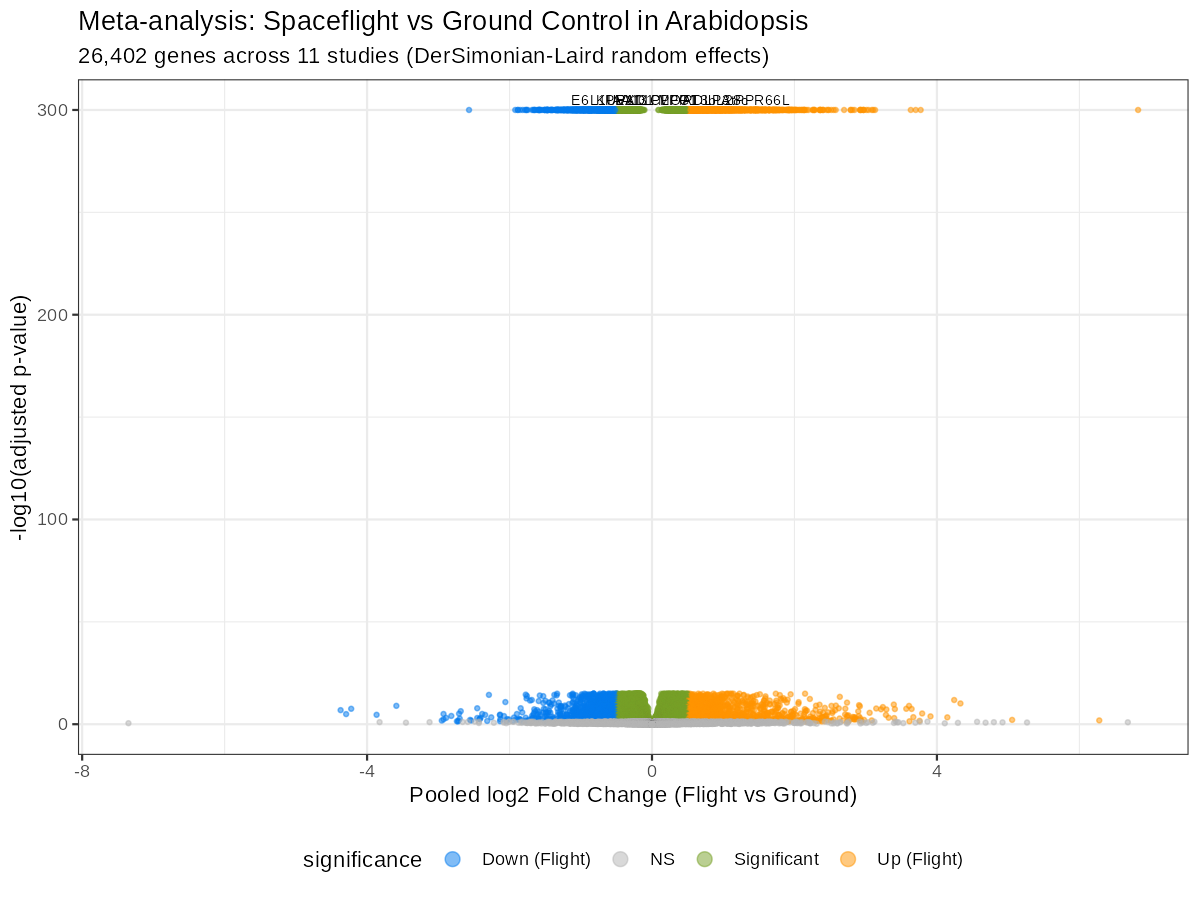
\includegraphics[width=0.95\textwidth]{../Figures/volcano_meta_analysis.png}
\caption{\textbf{Meta-Analysis Volcano Plot.}
$-\log_{10}(p)$ vs. effect size (log2FC) for 26,402 genes. Red points: padj $<$ 0.05. Top differentially expressed genes labeled. High heterogeneity ($I^2 > 80\%$) reflects cross-study variation.
}\label{fig:volcano}
\end{figure}

\begin{figure}[H]
\centering
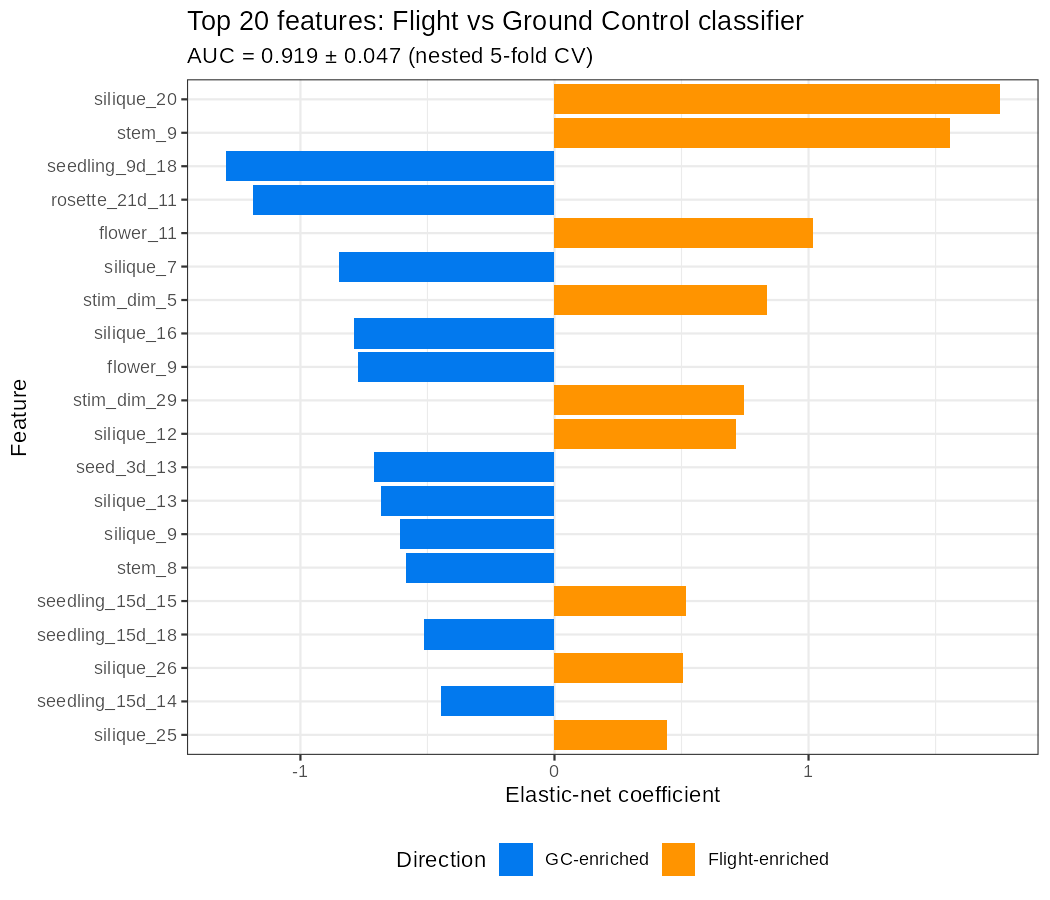
\includegraphics[width=0.95\textwidth]{../Figures/classifier_feature_importance.png}
\caption{\textbf{Flight vs Ground Control Classifier Feature Importance.}
Elastic-net regression coefficients for top 20 features (cell types and stimulus dimensions). stem\_9, seed\_425d\_7, and stimulus codes rank highest. AUC = 0.919 $\pm$ 0.047 (nested 5-fold CV).
}\label{fig:classifier_fi}
\end{figure}

\begin{figure}[H]
\centering
\begin{subfigure}[b]{0.48\textwidth}
  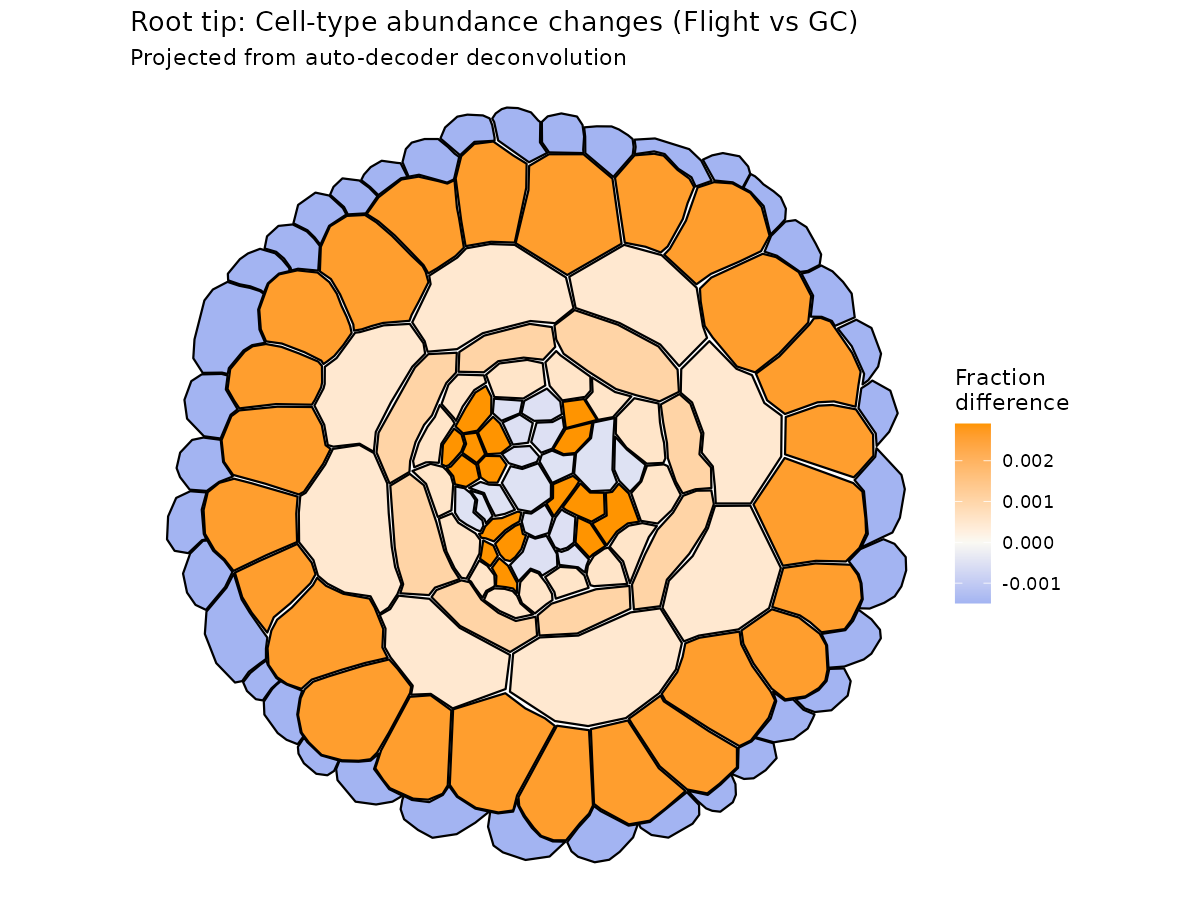
\includegraphics[width=\textwidth]{../Figures/ggplantmap_root_projection.png}
  \caption{Root tip cross-section}
\end{subfigure}
\hfill
\begin{subfigure}[b]{0.48\textwidth}
  \includegraphics[width=\textwidth]{../Figures/ggplantmap_shoot apex_projection.png}
  \caption{Shoot apex}
\end{subfigure}
\\
\begin{subfigure}[b]{0.48\textwidth}
  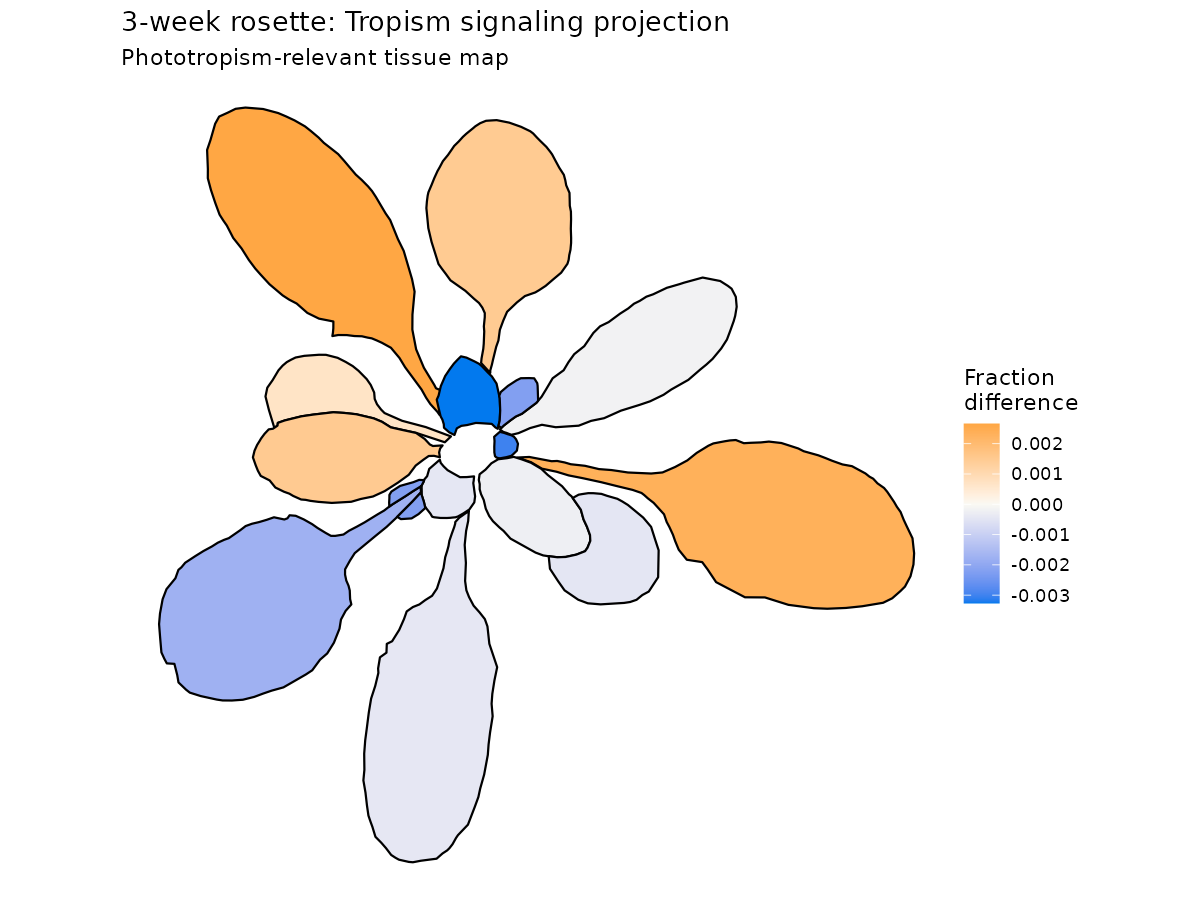
\includegraphics[width=\textwidth]{../Figures/ggplantmap_rosette_projection.png}
  \caption{3-week rosette}
\end{subfigure}
\hfill
\begin{subfigure}[b]{0.48\textwidth}
  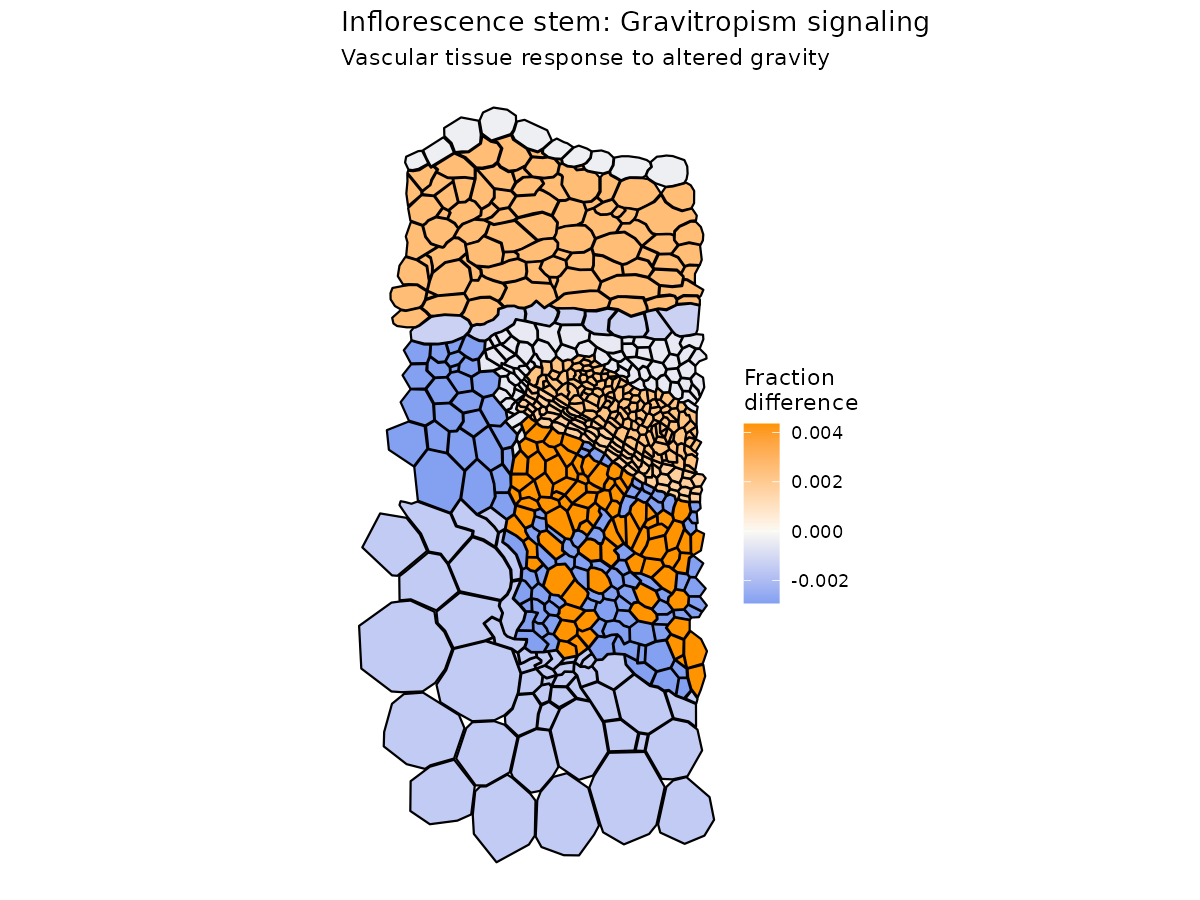
\includegraphics[width=\textwidth]{../Figures/ggplantmap_stem_crosssection.png}
  \caption{Stem cross-section}
\end{subfigure}
\caption{\textbf{ggPlantMap Tissue Projections of Cell-Type Spaceflight Response.}
Cell-type abundance changes mapped onto \Arabidopsis tissue anatomy. (a–d) Heat maps overlay deconvolution outputs (flight vs ground control log2FC per cell type) onto anatomical regions of interest (ROIs). Warm colors indicate elevated abundance in flight; cool colors, reduced. Inflorescence stem vascular regions (d) show strongest response.
}\label{fig:ggplantmap}
\end{figure}

\begin{figure}[H]
\centering
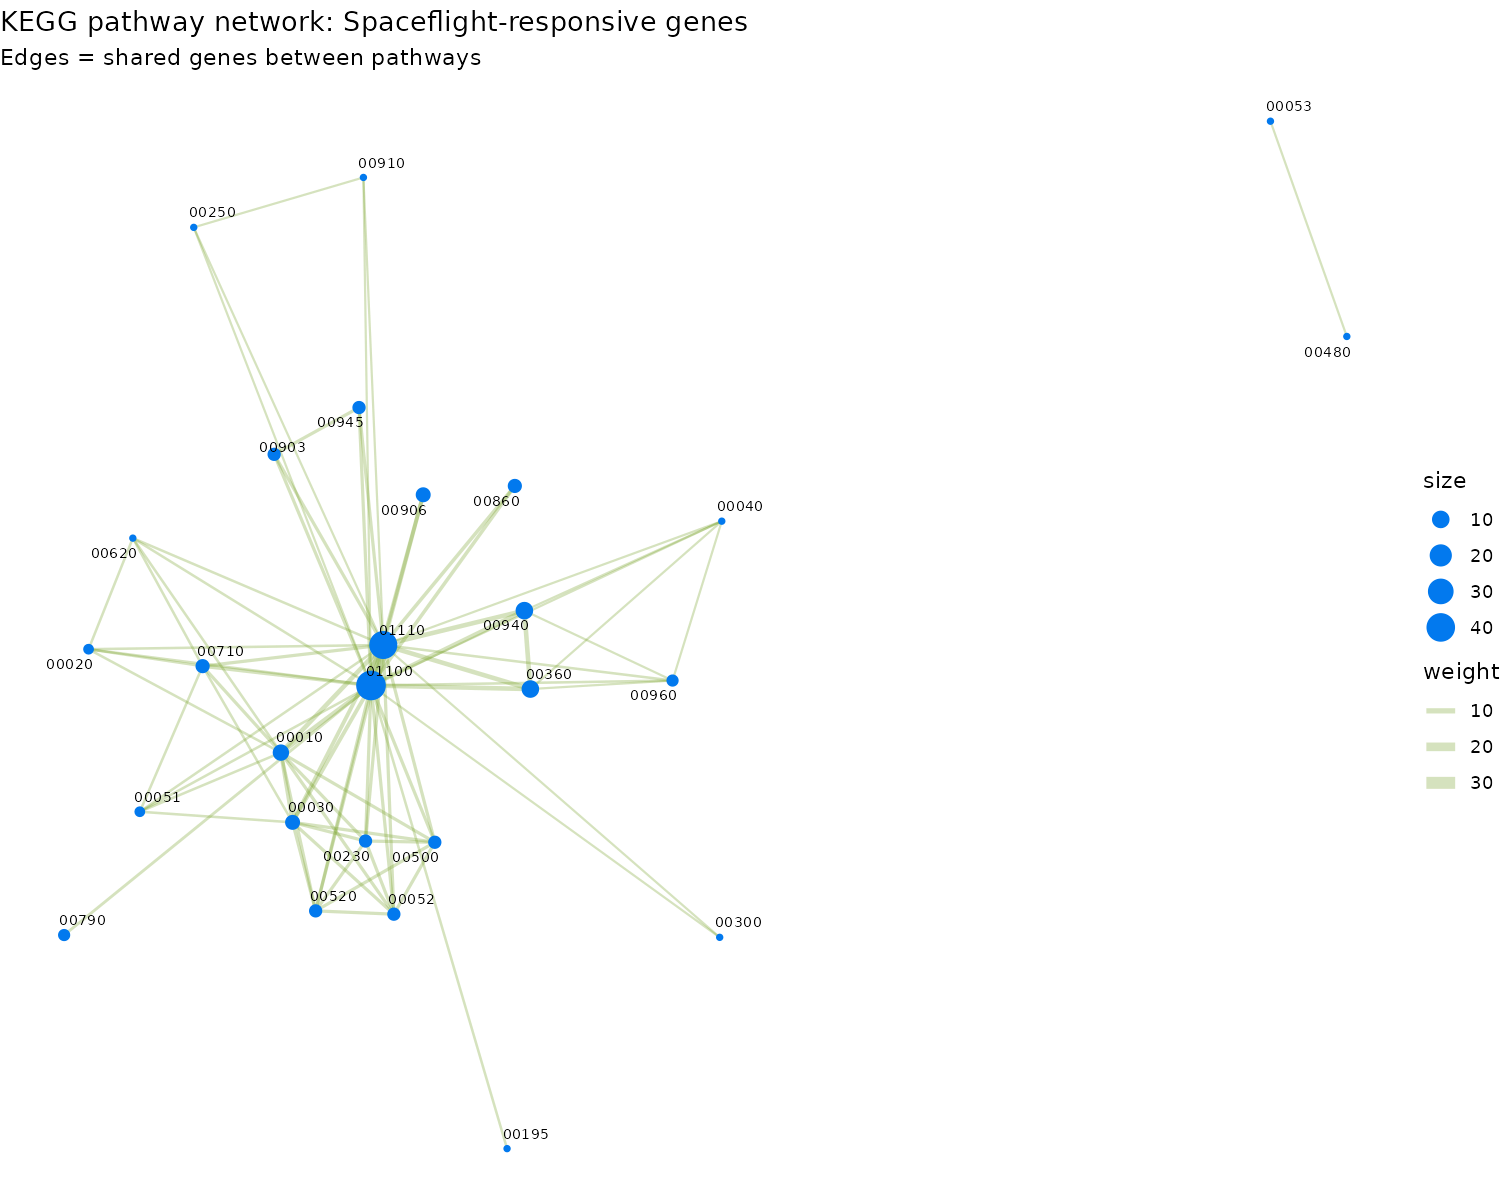
\includegraphics[width=0.95\textwidth]{../Figures/kegg_pathway_network.png}
\caption{\textbf{\KEGG Pathway Network of Differentially Expressed Genes.}
Network of pathways (nodes) connected by shared DE genes (padj $<$ 0.05). Node size indicates number of DE genes in pathway; edge thickness, number of shared genes. Central hubs include plant hormone signal transduction (ath04075) and carbon fixation (ath00710).
}\label{fig:kegg_network}
\end{figure}

\begin{figure}[H]
\centering
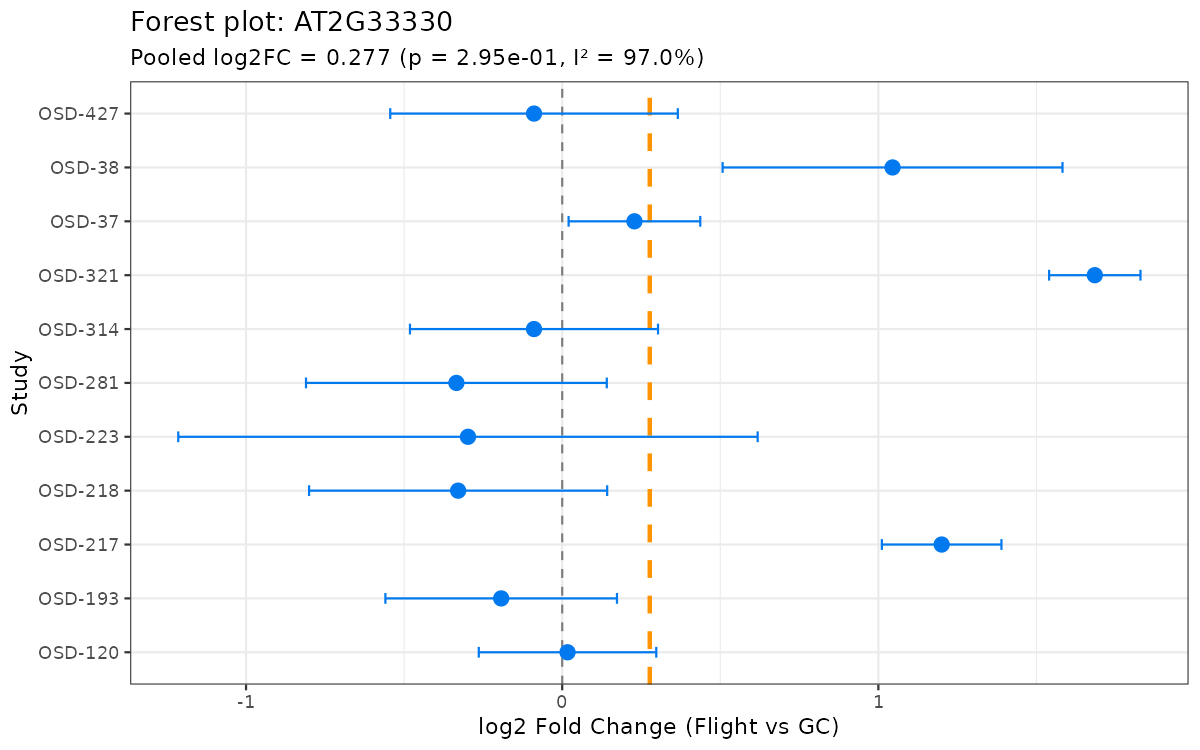
\includegraphics[width=0.95\textwidth]{../Figures/forest_plot_top_gene.png}
\caption{\textbf{Forest Plot: Top Meta-Analysis Gene Across 11 Studies.}
Shown is the forest plot for the top-ranked gene by $-\log_{10}(p)$ across 11 spaceflight studies. Each horizontal line represents study-specific log2FC with 95\% CI; the diamond is the random-effects meta-estimate. High heterogeneity ($I^2 > 80\%$) visible in wide individual CIs.
}\label{fig:forest}
\end{figure}

\begin{figure}[H]
\centering
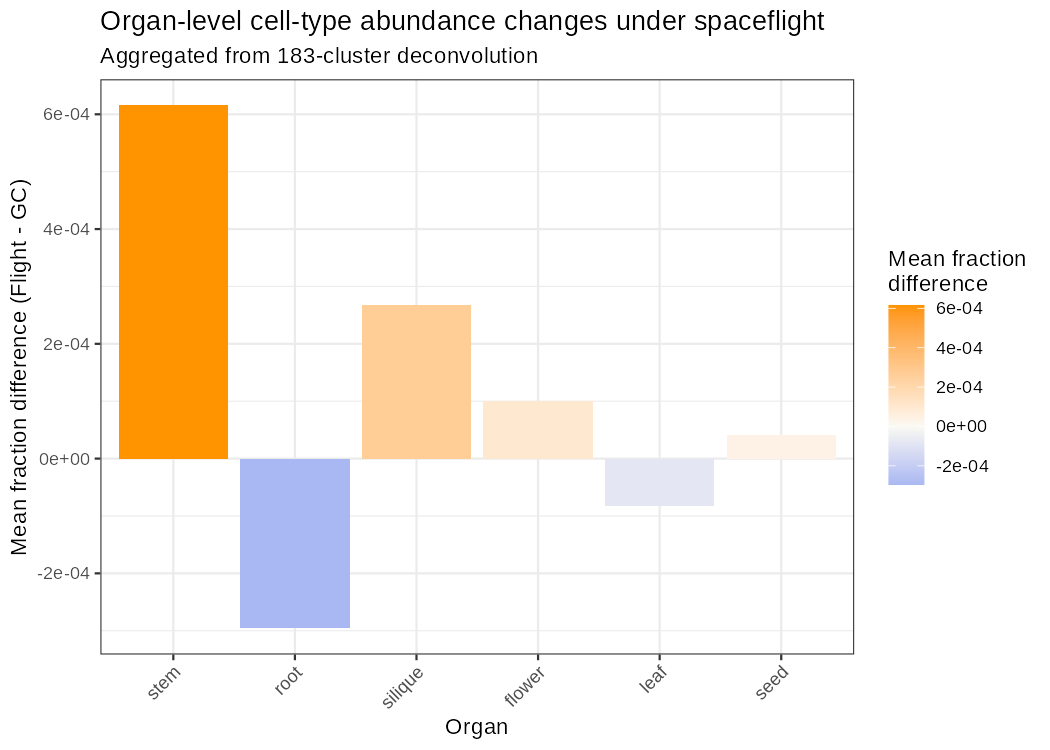
\includegraphics[width=0.95\textwidth]{../Figures/organ_level_diff_barplot.png}
\caption{\textbf{Organ-Level Abundance Changes in Spaceflight Samples.}
Mean cell-type fraction changes (flight minus ground control) aggregated by tissue. Root, rosette, shoot apex, leaf, and stem sampled. Inflorescence stem vascular clusters show largest magnitude changes. Error bars: SEM across samples per tissue.
}\label{fig:organ_barplot}
\end{figure}

\begin{table}[H]
\centering
\caption{\textbf{Key Results Summary.}}
\label{table:summary}
\begin{tabular}{lc}
\toprule
\textbf{Metric} & \textbf{Value} \\
\midrule
Total samples harmonized & 1,337 \\
\OSDR studies & 24 (18 RNA-seq + 6 microarray) \\
\GEO series & 6 \\
Atlas cells (foundation model) & 432,919 \\
Atlas clusters & 183 \\
Auto-decoder latent dimensions & 32 \\
Bulk samples deconvolved & 398 \\
DE studies (DESeq2) & 11 \\
Meta-analysis genes tested & 26,402 \\
Meta-analysis significant (padj $<$ 0.05) & 16,002 \\
Flight vs GC classifier AUC & 0.919 $\pm$ 0.047 \\
Tropism classifier F1 (grav. vs photo.) & 1.000 \\
Cell types with sig. spaceflight changes & 3 \\
\bottomrule
\end{tabular}
\end{table}

\end{document}
